\begin{center}\small
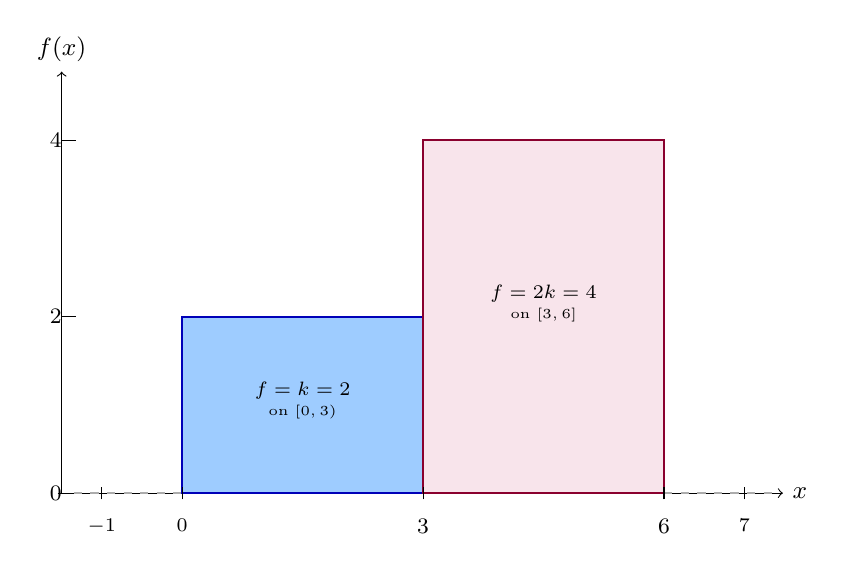
\begin{tikzpicture}[x=1.02cm,y=1.12cm]

  % Axes: $x\in[-1,7]$, $f$ up to $4$ (illustrative $k=2$)
  \draw[->] (-1.55, 0) -- (7.48, 0) node[right, font=\small] {$x$};
  \draw[->] (-1.5, 0) -- (-1.5, 4.78) node[above, font=\small] {$f(x)$};

  \foreach \yv in {0, 2, 4}{
    \draw (-1.5, \yv) -- (-1.32, \yv);
  }
  \foreach \yv/\Lb in {0/{$0$}, 2/{$2$}, 4/{$4$}}{
    \node[left=5pt, font=\footnotesize, inner sep=0pt] at (-1.32, \yv) {\Lb};
  }

  % Zero PDF on $(-\infty,0]$ and $(6,\infty)$ restricted to $[-1,0]$ and $[6,7]$
  \draw[thick, dashed, gray!65] (-1.35, 0) -- (0, 0);
  \draw[thick, dashed, gray!65] (6, 0) -- (7.4, 0);

  \fill[blue!52!cyan, opacity=0.38] (0, 0) rectangle (3, 2);
  \draw[thick, blue!72!black] (0, 0) rectangle (3, 2);

  \fill[purple!12, opacity=0.88] (3, 0) rectangle (6, 4);
  \draw[thick, purple!72!black] (3, 0) rectangle (6, 4);

  \foreach \xv in {-1, 0, 3, 6, 7}{
    \draw (\xv, -0.07) -- (\xv, 0.07);
  }

  \node[below=6pt, font=\scriptsize] at (-1, 0) {$-1$};
  \node[below=6pt, font=\scriptsize] at (0, 0) {$0$};
  \node[below=6pt, font=\footnotesize] at (3, 0) {$3$};
  \node[below=6pt, font=\footnotesize] at (6, 0) {$6$};
  \node[below=6pt, font=\scriptsize] at (7, 0) {$7$};

  \node[align=center, font=\scriptsize, inner sep=2pt] at (1.5, 1.05)
    {$f=k=2$\\[-1pt]{\tiny on $[0,3)$}};
  \node[align=center, font=\scriptsize, inner sep=2pt] at (4.5, 2.15)
    {$f=2k=4$\\[-1pt]{\tiny on $[3,6]$}};

\end{tikzpicture}\\[0.6em]

\noindent\footnotesize\textit{Illustration with $k=2$: steps at heights $k$ and $2k$; $f(x)=0$ on $[-1,0]$ and $[6,7]$. A valid pdf on $[0,6]$ needs $9k=1$, i.e.\ $k=\tfrac19$.}
\end{center}
